%% Typed Memory for Autonomous Agents
%%
%% Position / innovation paper, IEEE Transactions on Artificial Intelligence
%% register (IEEEtran journal mode). Built with `make` in this directory;
%% IEEEtran.cls is vendored under cls/ for the same reason acmart was.
%%
%% The earlier PVLDB experience-track formulation of this material is in the
%% repository history at commit 1c1372f and can be restored from it.
%%
%% RULES (unchanged from the experience version, and load-bearing here):
%%  - Every number was produced by a harness in this repository.
%%  - Numbers carrying a superscript p are prototype-era, from the Python
%%    predecessor, and are never presented as results of this system.
%%  - The todonum macro renders an unmeasured number in red; `make` counts
%%    uses of it and must report 0.

\documentclass[journal,nofonttune]{IEEEtran}

%% IEEEtran defaults to Times (ptm). That family ships in
%% texlive-fontsrecommended, which is not installed everywhere, and unlike
%% acmart's optional fonts its absence is a hard stop rather than a warning.
%% Fall back to Computer Modern so the build does not depend on an optional
%% package. Install texlive-fontsrecommended for camera-ready metrics.
\renewcommand{\rmdefault}{cmr}
\renewcommand{\sfdefault}{cmss}
\renewcommand{\ttdefault}{cmtt}
%% IEEEtran also hard-codes ptm as the family its save/restore pair falls
%% back to (IEEEtran.cls:4595), which \IEEEPARstart restores into.
\makeatletter
\gdef\@IEEESAVESTATEfontfamily{cmr}
\makeatother

\usepackage{booktabs}
\usepackage{balance}
\usepackage{xcolor}
\usepackage{amsmath}
\usepackage{tikz}
\usetikzlibrary{positioning, arrows.meta}
\usepackage{url}

%% An unmeasured number. Kept as the guard for future edits.
\newcommand{\todonum}[1]{\textcolor{red}{\textbf{[?~#1]}}}
%% A prototype-era number, inherited from the predecessor draft.
\newcommand{\pn}[1]{#1\textsuperscript{\textsf{p}}}
%% A cross-reference to the guarantee register.
\newcommand{\expref}[1]{\textsf{E-#1}}

\begin{document}

\title{Typed Memory for Autonomous Agents:\\
Co-Locating Schema, Instruction and Substrate\\
in One Authored Artifact}

\author{Joachim Rosskopf%
\thanks{J. Rosskopf is with DataZoo GmbH, Germany (e-mail:
jr@data-zoo.de).}%
\thanks{Figures marked \pn{x} are prototype-era, from a 430-line Python
predecessor and its verification record; they are never presented as results
of the system described here. All other figures were produced by harnesses in
the accompanying repository.}}

\markboth{IEEE Transactions on Artificial Intelligence}%
{Rosskopf: Typed Memory for Autonomous Agents}

\maketitle

\begin{abstract}
Retrieval-augmented agent memory is commonly organized as a vector index
over unstructured text, which offers no level of description between the
individual chunk and the whole corpus. Typed alternatives are not new: semantic
wikis, knowledge graphs and ontology-based data access have supplied schemas,
typed links and federated bindings for two decades. This paper argues that
what an agent needs is narrower and specific: the schema a record must
satisfy, the instruction a model executes when handling records of that kind,
and the declaration of where those records physically live, should be
\emph{one authored, versioned artifact} rather than three maintained
separately. We call such an artifact a \emph{skill}, and develop the
consequences. Discovery then enumerates authored types rather than generated
records; the same artifact that a curator edits is the one a model reads; and
a type library ships with its integrations, because the substrate binding is
a field of the type. State is maintained by projecting an immutable event log
through agent runs whose instructions are themselves such artifacts. We
report a 101{,}500-line implementation and three feasibility results: type
enumeration costs a fixed 744 tokens and sub-millisecond latency as the
corpus grows a thousand-fold; one navigation sequence reaches five
heterogeneous substrates from known handles; and event projection produced no
duplicate write across 35 process kills landing mid-write. These establish
that the arrangement is buildable and cheap to offer. They do not establish
that agents exploit it, which requires multi-type benchmarks with type-naming
queries that do not presently exist, and which we argue is the field's most
useful next contribution.
\end{abstract}

\begin{IEEEkeywords}
Autonomous agents, agent memory, knowledge representation, retrieval-augmented
generation, large language models, typed data models, event sourcing.
\end{IEEEkeywords}

%% =====================================================================
\section{Introduction}
\IEEEPARstart{S}{toring} a million facts has not been difficult for decades.
Placing the right handful of them into a bounded context window, repeatedly
and cheaply enough that an agent can afford to look, is what constrains
autonomous systems today. Every retrieval a language model performs is paid
for twice, in tokens and in turns, and both prices follow from one design
decision: how much the memory makes the agent read before it can decide what
to read next.

The most common answer is a vector index over chunked text. It answers one
question well---``what text resembles this text''---and charges a document
body for every answer. Structured alternatives exist and predate the current
interest in agents: knowledge graphs~\cite{kgsurvey}, semantic
wikis~\cite{semanticwiki}, collaboratively curated typed
entities~\cite{wikidata,schemaorg}, and tool schemas that constrain what a
model may call~\cite{toolformer}. Our argument is therefore not that
structure is missing from the field, but that the structure agents need is
distributed across artifacts that are maintained separately: a schema in one
place, the natural-language guidance a model follows in another, and the
mapping to where data physically resides in a third. Each is authored by
different people, versioned on different cycles, and reviewed by different
processes.

\textbf{Thesis.} Agent memory should be \emph{typed}; the types should be
authored by people and readable as instructions by models; and state should
be derived from an immutable event log by agent runs whose instructions are
themselves part of the typed corpus. Two dualities express this, and their
composition is the contribution.

\emph{Skill $\leftrightarrow$ Instance.} A skill page is at once the schema a
class of records must satisfy and the prose an agent reads to learn what that
class is for. An instance is at once a record of that type and a document a
person can edit. Discovery then operates over \emph{types}, which are
authored and therefore bounded in number, rather than over \emph{records},
which are generated and therefore not.

\emph{Event $\leftrightarrow$ Callback.} An event is an immutable fact; a
callback is an agent run that folds it into instance state, and the run's
instructions are the event's own skill page. State is a projection of the
log, so it is re-derivable, and an interrupted projection is replayable
rather than corrupting.

\textbf{A corollary with disproportionate practical weight.} Because the \emph{skill} declares its
storage backend, the substrate beneath an instance is a property of its type
rather than of the referent space. One type's instances are documents;
another's are rows of a read-only relational view; another's are chunks
extracted from an uploaded file; another's are fetched live from a remote
service on each read and accept writes back upstream. The agent reaches all
of them with the same navigation verbs. This is what allows a typed memory to
reason over an organization's data without first importing it.

\textbf{Contributions.}
\begin{enumerate}
\item A memory model for autonomous agents built on two dualities and a
  substrate corollary, with an explicit argument for why typing---not
  disclosure discipline alone---is what bounds context cost
  (Sections~\ref{sec:why}--\ref{sec:model}).
\item A realization of the model in 23 Rust crates and 101{,}500 lines,
  including the mechanisms it requires: index-time reference validation, a
  single embedded store for the index concerns, five instance backends behind
  one referent space, and a projection loop whose reducer generalizes from
  single-hop cascades to multi-phase fan-out
  (Section~\ref{sec:realization}).
\item A guarantee register of eighteen safety and semantic properties in
  which every row names an integration test that executes in the project's
  ordinary test run (Section~\ref{sec:guarantees}).
\item Evidence for three claims of the model, and an explicit account of four
  experiments we specify and do not run, with what each would settle
  (Sections~\ref{sec:evidence}--\ref{sec:open}).
\end{enumerate}

The fourth item is stated as a contribution because the unrun experiments
bound the claims of the first three, and a reader cannot calibrate the
position without them.

%% =====================================================================
\section{Why Untyped Memory Does Not Scale}
\label{sec:why}

\subsection{A Cost Model}
An agent's cost on a task is the tokens carried in context multiplied by the
turns taken, and both follow from how much the memory requires it to read
before acting. Following the progressive-disclosure principle introduced for
procedural knowledge~\cite{agentskills}, we distinguish \emph{Tier 1}, the
metadata loaded at cold start, from \emph{Tier 2}, the bodies subsequently
retrieved.

\subsection{A Chunk Index Has a Weak Tier 1}
Tier 1 requires something enumerable and small. A chunk index can offer
collections, namespaces, directory structure, tags or generated summaries, so
it is not literally without metadata; but none of these is a \emph{contract}
that records are validated against, and none carries guidance a model can act
on. What an agent can enumerate is therefore either too coarse to select on
or too numerous to hold. A vocabulary of authored types supplies both
properties at once: it is small because people write it, and it is
actionable because each entry states what records of that kind are for.

Table~\ref{tab:costmodel} gives the resulting arithmetic, measured on the
predecessor system's corpora. The absolute figures are prototype-era; the
ratio is the point. At ten thousand pages, reading metadata alone costs three
to five thousand tokens and reading every page costs four to six hundred
thousand, while enumerating \emph{types} costs a constant independent of the
corpus.

\begin{table}[!t]
\caption{Cold-start cost by disclosure strategy. Prototype-era measurements,
\texttt{tiktoken cl100k\_base}, against a nominal 30k working budget.}
\label{tab:costmodel}
\centering
\begin{tabular}{lrr}
\toprule
strategy & 10k pages & 100k pages \\
\midrule
every page, full content          & \pn{400--600k} & \pn{4--6M} \\
every page, metadata only         & \pn{3.2--4.8k} & \pn{8--12k} \\
every \emph{type}, metadata only  & \pn{189}       & \pn{189} \\
\bottomrule
\end{tabular}
\end{table}

\subsection{Where the Binding Lives}
A vector index reasons only over text already ingested, so tables, archived
files and records behind service interfaces must be copied in and chunked;
the copy is stale on arrival and the refresh pipeline is a component somebody
operates. Federated approaches solve exactly this. Ontology-based data access
and virtual knowledge graphs~\cite{obda} expose remote sources through a
common vocabulary without copying, as do dataspaces~\cite{dataspaces} and
linked data~\cite{linkeddata}. Our claim is not that federation is missing
but that the \emph{mapping} is conventionally an engineering artifact held
apart from the vocabulary---authored in a mapping language, deployed by a
different team, invisible to whatever instructs the consumer. Placing the
binding in the type changes what can be distributed: a vocabulary and its
integrations become one versioned object, discussed in
Section~\ref{sec:packs}.

\subsection{Longer Contexts Do Not Resolve It}
Large context windows make the naive strategy feasible at small scale and
still inadvisable. Cost and latency grow with the window, and retrieval
accuracy degrades for material in its middle~\cite{lostmiddle}. More
fundamentally the strategy has no stable operating point: a corpus that fits
today does not fit next year, and the failure is silent.

\subsection{Writes Without Schemas Accumulate Contradictions}
The write path of an untyped memory is ``embed and append.'' Nothing
validates new material, marks what it supersedes, or links it to the entities
it concerns. Contradictions accumulate at exactly the rate content does, and
a layer that ranks by similarity cannot prefer the correct one of two similar
answers.

\subsection{Typed Memory Without a Loop Goes Stale}
The complement is equally damaging. A typed knowledge base with no ingestion
loop is a wiki: correct when written, quietly wrong some weeks later, and
trusted considerably longer. A model of agent memory that stops at the data
model has described half a system, which is why the model below has two
dualities rather than one.

%% =====================================================================
\section{The Two-Duality Model}
\label{sec:model}

\subsection{Skill $\leftrightarrow$ Instance}
The starting observation is structural: an agent-skill page and a typed wiki
note are the same artifact---text with structured frontmatter, an identifier
and a description---differing only in whether the reader treats the content as
instructions or as data. Letting an instance declare which skill it conforms
to makes that skill its type, and makes the instruction and the schema the
same page.

A corpus is a set of pages $P = S \cup I$ with $S$ the skills and $I$ the
instances, a total function $\tau : I \rightarrow S$ given by each instance's
declared type, and a typed reference relation $R \subseteq P \times S \times
P$ in which $(p, s, q) \in R$ requires $\tau(q) = s$. The requirement is
checked when a page is indexed rather than when a reference is followed,
which makes a dangling or mistyped reference a reportable error instead of a
runtime surprise.

\textbf{Why this bounds context cost.} Discovery enumerates $S$, not $I$. $S$
is authored by people---it is the vocabulary of a domain, not its
contents---so its cardinality is bounded by human attention rather than by
ingestion rate. A tenant ingesting a million meeting records still has one
\texttt{meeting} type. The precision matters: progressive disclosure bounds
cost \emph{only because} typing supplies a level of description at which to
stop. Applied to an untyped corpus, disclosure has nothing to disclose about.

Concretely, an agent asked what changed for a customer last quarter first
enumerates types, receiving on the order of a hundred identifier-description
pairs and no bodies. It selects two, issues one listing filtered by type and
date range, and expands the two or three records it needs. The remaining
records cost nothing, because no step in that sequence has a size depending
on how many exist.

\subsection{References Carry Type, Locus and Version}
A reference splits on alias, anchor, version and type separators, yielding
six usable forms from a bare type reference to
\texttt{[[type::id\#anchor@version|alias]]}. The anchor addresses a block
within a record; the version pins a snapshot, so a reference into external
versioned data denotes the same bytes indefinitely. Typing also removes an
ambiguity untyped wiki references leave open: in the predecessor,
\texttt{[[Anna Mueller]]} and \texttt{[[anna-mueller]]} resolved to two
distinct nodes because nothing defined a canonical form.

\subsection{The Corollary: the Type Declares the Substrate}
\label{sec:corollary}
Skills carry a backend declaration, and it is the skill that carries
it---never the individual instance, never the caller. Five substrates are
realized here: native documents, a read-only relational view over an external
database, an extracted and chunked binary file, a live remote service, and a
live upstream tool server. The last two hold no local copy: the body is
fetched on each read and edits are forwarded upstream.

One invariant makes this inexpensive. Every external instance retains a
native overlay page, which \emph{is} the instance as far as the referent
space is concerned---identity, references, access control and history reuse
existing machinery---while a binding record connects it to the external data.
All novelty is confined to where the body originates, which is why adding a
substrate required no change to the dispatcher, the wire format, or the
reading agent's vocabulary.

One division shows through, and we state it rather than claim a transparency
the model does not have: materialized substrates are indexed and therefore
reachable by similarity, whereas live proxies are not. A remote instance is
reachable by reference, not by resemblance.

\subsection{Event $\leftrightarrow$ Callback}
An event is an instance of an event-typed skill carrying a timestamp and
typed references to what it concerns. Events are immutable by convention: a
correction is a new event citing the original, not an edit. The inbox is the
unprojected suffix of the log.

When an event arrives, a runner triggers an agent harness whose task
description \emph{is} the event's labelling skill page and whose tool surface
is the ordinary agent API. There is no per-harness client and no prompt
template maintained outside the corpus: the instructions for processing a
class of event live in that class's type, where they are read, reviewed and
versioned like any other page.

State therefore lives in the knowledge base rather than in an orchestrator's
variables. This inversion is what makes the loop recoverable: an engine
holding progress in local memory loses it when the process dies, whereas a
projection over a durable log resumes by re-reading what it already wrote.

\subsection{Composition}
The dualities are not independent contributions sharing an implementation;
each supplies something the other requires. The skill-as-schema is what a
callback's write is validated against, and the skill-as-prompt is what drives
the callback at all. The event is an instance's provenance; the callback is
how the instance acquires a current value. The substrate corollary lets the
loop reach beyond the corpus: because an instance may be a live remote
record, a callback can fold an event into a system the memory does not own,
writing through rather than into a copy that will drift.

Remove the corollary and the model still functions, but only over material
already imported---which is where most retrieval-augmented architectures sit,
and why so much of their engineering is pipeline engineering.

\begin{figure}[!t]
\centering
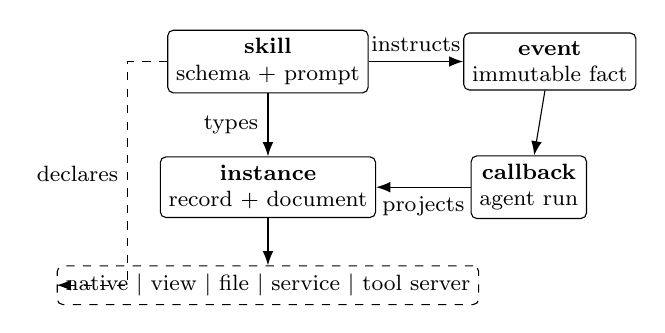
\begin{tikzpicture}[
  font=\footnotesize,
  box/.style={draw, rounded corners=2pt, align=center, inner sep=3pt,
              minimum height=6mm},
  sub/.style={draw, dashed, rounded corners=2pt, align=center, inner sep=3pt},
  ar/.style={-{Latex[length=1.8mm]}}
]
\node[box] (skill) {\textbf{skill}\\schema $+$ prompt};
\node[box, below=8mm of skill] (inst) {\textbf{instance}\\record $+$ document};
\node[box, right=12mm of skill] (event) {\textbf{event}\\immutable fact};
\node[box, right=12mm of inst] (cb) {\textbf{callback}\\agent run};
\draw[ar] (skill) -- node[left] {types} (inst);
\draw[ar] (event) -- (cb);
\draw[ar] (skill) -- node[above] {instructs} (event);
\draw[ar] (cb) -- node[below] {projects} (inst);
\node[sub, below=6mm of inst] (subs)
  {native $\vert$ view $\vert$ file $\vert$ service $\vert$ tool server};
\draw[ar] (inst) -- (subs);
\draw[ar, dashed] (skill.west) -- ++(-5mm,0) |-
  node[left, pos=0.25] {declares} (subs.west);
\end{tikzpicture}
\caption{The model. A skill types its instances and instructs the callback
handling events of that kind; an event fires a callback, which projects it
into instance state. The substrate beneath an instance is selected by the
\emph{skill}, never by the caller.}
\label{fig:model}
\end{figure}

%% =====================================================================
\section{What Is and Is Not New Here}
\label{sec:novelty}

Each element of the model has precedent, and it is worth stating plainly
which. Typed records with human-authored schemas and typed links are the
substance of semantic wikis~\cite{semanticwiki} and of collaboratively curated
entity bases~\cite{wikidata,schemaorg}. Exposing heterogeneous sources through
one vocabulary without copying is ontology-based data access and virtual
knowledge graphs~\cite{obda}, anticipated by dataspaces~\cite{dataspaces} and
linked data~\cite{linkeddata}. Deriving state by folding an immutable log is
event sourcing~\cite{eventsourcing}. Constraining what a model may invoke by a
schema is standard tool use~\cite{toolformer}. None of these is claimed as a
contribution.

The claim is about \emph{co-location}. In the systems above, three artifacts
are maintained separately: the schema a record satisfies, the guidance a
consumer follows when handling records of that kind, and the mapping from the
vocabulary to physical storage. An ontology does not tell an agent what to do
with an instance; a mapping file is invisible to whatever does; and the prose
that guides a human curator lives in a manual. This paper's position is that
for agent memory the three should be one authored page, and that three
consequences follow which do not follow from any of them separately.

\emph{Curation and instruction become the same act.} Editing what a type means
edits what the agent does with it, in the same review, with the same version
history. There is no drift between an ontology and the prompt that consumes
it, because there is no prompt outside the corpus.

\emph{Discovery and specification become the same enumeration.} The set an
agent lists at cold start is the set a curator maintains. Its cardinality is
therefore governed by human attention rather than by ingestion rate---the
property Section~\ref{sec:evidence} measures---and it cannot silently diverge
from the schema, because it is the schema.

\emph{Vocabulary and integration become one distributable object.} Because the
substrate binding is a field of the type, a type library ships with the means
of resolving its instances against a subscriber's own systems
(Section~\ref{sec:packs}). Ontology-based access separates these by design,
which is appropriate when the ontology is a shared standard and awkward when
the vocabulary is a working artifact of one organization.

A reasonable objection is that co-location is an implementation convenience:
a callback could equally be driven by code, a policy file or a tool schema
outside the corpus. That is true, and it is why we do not claim the
arrangement is necessary. We claim it is consequential, and
Section~\ref{sec:evidence} reports what it costs to offer; whether it changes
agent behaviour is the open question of Section~\ref{sec:open}.

%% =====================================================================
\section{Realization}
\label{sec:realization}

A model of this kind is interesting only if it can be built without the
mechanisms quietly reintroducing the costs it claims to remove. We describe
an implementation, in 23 Rust crates and approximately 101{,}500 lines, that
realizes each element.

\subsection{One Embedded Store for the Index Concerns}
Each tenant is a document directory beside a single embedded analytical
database file~\cite{duckdb}. That file carries relational metadata and the
typed reference graph; a block table whose vector column is indexed by HNSW
and whose text column by BM25; the operation log of the collaborative editing
layer; and an attachment point for read-only lakehouse
catalogs~\cite{ducklake}. A type-filtered vector query is consequently a
single SQL statement, because the filter columns are denormalized alongside
the vector.

The document directory remains canonical and everything in the database is
derivable from it. This keeps a typed memory inspectable by ordinary tools:
version control still diffs the corpus, text editors still edit it, and
recovery is a rebuild rather than a restore.

\subsection{Validation at Index Time}
Reference parsing is by regular expression rather than an AST walk, because
document parsers split reference delimiters across nodes in ways depending on
surrounding context. Four checks run in the same pass---the type exists, the
target exists, the target's declared type matches the reference, and any
named anchor is present---and their output is the same issue list the
validation API returns for a dry run, so an authoring agent receives exactly
the feedback the indexer would give, before it writes.

\subsection{One Referent Space, Five Substrates}
\label{sec:substrates}
The corollary is where an implementation makes outbound network calls on
behalf of tenant-authored content, so its safety properties belong to the
design rather than to operations. Credentials are registered out of band and
never appear in the corpus. A remote type names an administrator-registered
endpoint rather than a URL, so tenant-authored text cannot direct the system
at an arbitrary host, and a declared kind disagreeing with the registered
kind fails closed. A read that times out returns the overlay page with an
explicit issue marker rather than a partial body. Write-back templates are
bound by value, and an unresolvable placeholder aborts the call rather than
transmitting a literal. A relational binding records a fingerprint of its
source schema and revalidates it, marking the binding degraded when the
source has moved beneath it.

\subsection{The Projection Loop}
All automation resides outside the knowledge base. A separate runner
subscribes to an outbound notification and also polls the inbox---the poller
being the self-healing path for a missed notification---and both converge on
one bounded queue per tenant. A durable ledger, deliberately outside the
tenant store, records one row per run and is the basis of idempotency,
deduplication, depth and budget limits, and cycle detection.

The cascade emitter is already a reducer over a run's event log, though a
degenerate one: it emits at most one follow-on event per confirmed cross-type
write and performs no join. A multi-phase workflow is the same reducer with
three parameters raised---an explicit plan read from a workflow type, fan-out
width greater than one, and a quorum barrier. We note this because fan-out
orchestration is widely built as a second execution model beside a reactive
one, and the model suggests it need not be: invoking a workflow is itself an
inbox event, and the only thing distinguishing it from an externally captured
one is which party captured it.

\subsection{Types as Distributable Artifacts}
\label{sec:packs}
Because types are documents, they are distributable. A pack is a versioned,
read-only layer to which a tenant subscribes; local pages shadow base pages
of the same name, promotion into the base layer passes a curator gate, and a
pinned version does not move on its own. With the substrate corollary in
play, a pack ships more than a schema: a customer-management pack carries
types whose instances resolve against \emph{the subscriber's} registered
endpoint, so vocabulary and integration arrive together and the subscriber
supplies only a credential. We regard this as the model's most consequential
implication for practice, and the least explored.

%% =====================================================================
\section{Guarantees}
\label{sec:guarantees}

A memory system is a contract, and a contract not written down is one the
next component will violate. Table~\ref{tab:guarantees} states eighteen
properties, each verified by an integration test executing in the project's
ordinary test command; none is disabled, because a claim whose test does not
run is not a claim. An untyped vector store provides none of these except a
durable append: it has no typed reference to resolve, no schema to validate
against, no session to converge and no binding to degrade.

\begin{table}[!t]
\caption{The guarantee register. Each row names a test executing in the
project's ordinary test run.}
\label{tab:guarantees}
\centering
\footnotesize
\begin{tabular}{ll}
\toprule
 & property \\
\midrule
\expref{1} & typed reference resolution is deterministic and total \\
\expref{2} & a reference failing any of four checks is reported \\
\expref{3} & anchors and versions survive resolution unchanged \\
\expref{4} & concurrent editing sessions on one page converge \\
\expref{5} & a mid-write crash rolls back every table together \\
\expref{6} & the index is reproducible from documents alone \\
\expref{7} & a stale base version is rejected, not silently merged \\
\expref{8} & one event yields exactly one terminal run \\
\expref{9} & a cascade terminates on depth or cycle detection \\
\expref{10} & a workflow phase completes only at barrier quorum \\
\expref{11} & non-native substrates refuse page-level writes \\
\expref{12} & subscribed base pages cannot be written or forged \\
\expref{13} & credentials never appear in the corpus \\
\expref{14} & a remote read fails closed on kind mismatch \\
\expref{15} & an unreachable endpoint degrades, never fabricates \\
\expref{16} & an unresolvable write placeholder aborts upstream \\
\expref{17} & source schema drift marks the binding degraded \\
\expref{18} & a token minted for another tenant is refused \\
\bottomrule
\end{tabular}
\end{table}

The eighteenth property illustrates what a register is for. Our specification
describes a tenant manager holding per-tenant handles; it is not implemented,
and the deployed isolation boundary is the process rather than a structure
inside it. Authentication resolved a tenant from the presented token while
the data path used the served tenant, and for some weeks the two were not
compared, so a validly signed token for one tenant was accepted against
another. A test had encoded the defect as intended behaviour: a foreign token
succeeding was being used to demonstrate that quota accounting was
per-tenant. Writing the contract down forced the comparison that exposed it.

%% =====================================================================
\section{Evidence}
\label{sec:evidence}

We report evidence for three claims. All measurements come from harnesses in
the accompanying repository, each taken in a single session on one machine,
since cross-session ratios are artifacts. No claim about agent behaviour is
advanced, because no experiment here measures it.

\subsection{Discovery Cost Is Invariant in Corpus Size}
Table~\ref{tab:tier1} measures cold-start cost over a synthetic tenant with
24 authored types and instance counts spanning $10^2$ to $10^5$. Instances
are inserted in bulk, as the quantity under test is a read.

\begin{table}[!t]
\caption{Tier-1 cost against corpus size. Tokens are
\texttt{cl100k\_base}; latency is 30 samples per column.}
\label{tab:tier1}
\centering
\footnotesize
\begin{tabular}{lrrrr}
\toprule
instances & $10^2$ & $10^3$ & $10^4$ & $10^5$ \\
\midrule
Tier-1 tokens         & 744 & 744 & 744 & 744 \\
Tier-1 p50 (ms)       & 0.74 & 0.74 & 0.76 & 0.81 \\
Tier-1 p95 (ms)       & 0.88 & 0.91 & 0.80 & 1.16 \\
whole corpus (tokens) & 2.9k & 29k & 290k & 2.9M \\
ratio avoided         & 3.9$\times$ & 39$\times$ & 390$\times$ & 3898$\times$ \\
\bottomrule
\end{tabular}
\end{table}

Part of this is arithmetic rather than discovery, and we say so: the
enumeration query selects on page type and cannot observe instances, so the
payload could not have varied. Its value is as a guard---the harness asserts
the equality, so if discovery ever begins to touch instances a test fails
rather than a claim quietly becoming false.

The open question was latency, since discovery shares a table with every
instance and the scan could have degraded. Across a thousand-fold increase in
corpus size it moves from 0.74 to 0.81\,ms at the median, roughly ten
percent, while the material it declines to read grows to 2.9\,M tokens.

\subsection{One Navigation Sequence, Five Substrates}
Table~\ref{tab:substrates} reports the same entity described by five types,
one per substrate, against a containerized relational database, an extracted
binary file, a live remote service and a live upstream tool server. The same
sequence---resolve, expand, traverse---runs against each.

\begin{table}[!t]
\caption{One entity on five substrates; 50 samples per latency cell, one
session. Search is each type's \emph{declared} capability, not a probe.}
\label{tab:substrates}
\centering
\footnotesize
\setlength{\tabcolsep}{3pt}
\begin{tabular}{lccccc}
\toprule
 & native & view & file & service & tool \\
\midrule
navigation steps ok & 3/3 & 3/3 & 3/3 & 3/3 & 3/3 \\
declared search     & hybrid & late & hybrid & none & none \\
expand p50 (ms)     & 3.8 & 9.4 & 5.8 & 6.7 & 6.5 \\
expand p95 (ms)     & 4.7 & 10.2 & 6.9 & 8.3 & 7.7 \\
payload (bytes)     & 380 & 760 & 1572 & 436 & 427 \\
\bottomrule
\end{tabular}
\end{table}

All fifteen navigation steps succeed: one set of verbs, in one order, routed
to a local file, a relational query, a chunked document and two live
services. Two limits bound the claim. The caller is not blind to the
substrate---the type segment of a reference names it, which is the design,
since it is the type that declares the backend---so what is identical is the
call shape rather than the caller's ignorance. And each instance is addressed
by a handle obtained at creation, so this establishes navigation rather than
discovery of an arbitrary entity.

Discoverability is read from each type's declaration rather than probed. A
probe would have been invalid here: the fixture runs a zero-vector embedder,
under which every vector is identical and search returns essentially the whole
corpus. The declarations divide as the design specifies, with live proxies
reporting no search capability. This row is therefore configuration
inspection, not a behavioural measurement, and is included only to document
where the abstraction is deliberately incomplete.

The latency ordering runs contrary to the intuition that materialized
substrates answer locally in single-digit milliseconds while live proxies
exhibit a network round trip. The relational view is instead the slowest
column at 9.4\,ms, half again the cost of either proxy, because every read
crosses into the external database while the proxies were answered by loopback
services in the same process. Two consequences follow. The proxy figures are a
floor excluding real network latency. And \emph{materialized does not imply
local}: a relational view is a live query behind a materialized interface, a
distinction the design documentation blurred and this measurement does not.
The ordering is descriptive of one session---50 warm calls, no independent
repeats, single-digit millisecond gaps---but its direction is the opposite of
the prediction.

\subsection{Projection Produced No Duplicate Write Under Failure}
Table~\ref{tab:loop} drains twenty events to quiescence under three
configurations; Table~\ref{tab:replay} reports recovery from process failure.
Measurement uses a deterministic stand-in for the language model, so the
figures describe the loop rather than inference latency.

\begin{table}[!t]
\caption{Twenty events drained to quiescence, one session. The clock starts
after capture. The arms are not a clean isolation: lifting the governor also
changes the failure profile.}
\label{tab:loop}
\centering
\footnotesize
\begin{tabular}{lccc}
\toprule
 & governed & lifted & lifted \\
target instances & 1 & 1 & 20 \\
\midrule
seconds to quiescence  & 9.17 & 9.66 & 9.87 \\
events per second      & 2.18 & 2.07 & 2.03 \\
ledger runs per event  & 1.25 & 1.75 & 1.75 \\
stopped by a control   & 5 & 5 & 5 \\
runs recorded failed   & 10 & 0 & 0 \\
max folds of one event & 1 & 1 & 1 \\
\bottomrule
\end{tabular}
\end{table}

Two candidate explanations for the throughput bound are unsupported in this
fixture. The per-tenant governor admits 120 runs per minute over a fixed
window, which averages two per second; raising it to 100{,}000 changed
throughput not at all, so admission control is not the binding constraint
here. Write contention is the second candidate, since all twenty events
folded into one page behind a per-tenant write lock; giving each event its
own target changed nothing either. Because the arms are not a clean
isolation---lifting the governor also changes the failure profile---these are
non-results rather than falsifications. What remains is an undecomposed
residual of roughly 475\,ms per event; the harness times quiescence, not its
components, so the serial per-run cost this suggests is a hypothesis. One
side effect is measurable: lifting the governor moved runs recorded failed
from ten to none at identical throughput, indicating it converts contention
into retries rather than into delay.

\begin{table}[!t]
\caption{Recovery from process failure, 100 trials, kill point sampled from a
deterministic sequence in $[20,100]$\,ms. Only the in-flight row tests
replay.}
\label{tab:replay}
\centering
\footnotesize
\begin{tabular}{lcc}
\toprule
kill landed & trials & converged \\
\midrule
before the run started   & 0  & --- \\
\textbf{while in flight} & \textbf{35} & \textbf{35} \\
after the run completed  & 65 & 65 \\
\midrule
duplicate folds & \multicolumn{2}{c}{0} \\
never processed & \multicolumn{2}{c}{0} \\
\bottomrule
\end{tabular}
\end{table}

The experiment requires a kill point that lands inside the write window, and
verifying this is not optional: a first configuration sampling from a wider
interval produced a hundred percent convergence in which \emph{every} kill
landed after the run had already completed, and therefore measured nothing.
Instrumenting the kill phase and narrowing the interval placed 35 of 100
kills genuinely in flight. All 35 converged, with no duplicate projection and
no event left unprocessed. The denominator is 35, not 100, and it bounds the
duplicate rate loosely; a rare interleaving would not appear at this sample
size. The result is also obtained with a deterministic stand-in for the
language model, which removes the component most likely to lengthen the
failure window, so it should not be read as an exactly-once guarantee in the
distributed-systems sense.

\subsection{Retrieval Mechanics}
For completeness we report the retrieval ladder over a public benchmark
(SciFact, 5{,}183 documents, 300 queries,
\texttt{bge-base-en-v1.5}): single-pass retrieval attains nDCG@10 of 0.723
and recall@100 of 0.976 at a median 141\,ms, while a two-pass variant using a
128-dimensional coarse pass attains 0.718 and 0.976 at 182\,ms. The
optimization does not pay at this corpus size: 29\% additional median latency
and a third of throughput for identical recall. The measured latency is
dominated by CPU query encoding rather than index search, making it a useful
figure for an agent's round trip and a misleading one for the index.

This benchmark cannot speak to the model's central claim. A public IR corpus
has no type structure, so a type-filtered query and an unfiltered one are the
same query.

%% =====================================================================
\section{What This Does Not Establish}
\label{sec:open}

Four experiments are specified in the accompanying repository and were not
run. Each is stated because their absence bounds the claims above.

\textbf{Whether an agent exploits the cheap tier.} This is the behavioural
half of the central claim and the most important gap. Table~\ref{tab:tier1}
shows the mechanism is available at fixed cost; it does not show that a
language model reads descriptions, selects a type, and expands two records
rather than twenty. The predecessor's real-model run reached correct answers
in \pn{1--2} tool calls at \pn{12.4}$\times$ lower token cost than a flat
baseline on a twenty-page corpus, reported here as prototype context and not
as a result for this system. A three-arm comparison against flat retrieval
and whole-corpus prompting, at several scales, would settle it.

\textbf{Whether typing improves retrieval quality.} Separating the
contribution of typing from that of metadata filtering requires a multi-type
corpus with queries naming a type. No public benchmark we are aware of
provides one. Constructing a synthetic corpus is possible and we regard it as
the necessary next step; we did not attempt it here because a benchmark whose
type partitioning is chosen by the authors of the system under test invites
an obvious objection, and answering that objection requires a construction
protocol agreed beyond one group. This bounds the present paper to a
feasibility claim.

\textbf{Whether the type count stays bounded.} This is the falsifier: if
authored types grow proportionally with generated records, discovery ceases
to be cheap and the model fails. Establishing it requires corpus histories
from long-running deployments in a form we can publish. We declined to
substitute a curve drawn from example fixtures, since for this claim
especially an unconvincing figure is worse than an acknowledged absence.

\textbf{Whether storage consolidation cost retrieval quality.} Thresholds
were declared in advance before merging retrieval and relational state into
one store; the labelled corpus against which they were declared was never
versioned alongside the code and no longer exists. We record this as a
process finding: an acceptance gate whose fixture is not versioned with the
system is a gate still open at deployment.

Two negative results also bear recording. Lexical retrieval collapsed to
\pn{0.350} nDCG on a duplicate-stress corpus where vector retrieval held at
\pn{0.933}, contradicting the expectation that BM25 degrades gracefully under
near-duplication. And the encoder our own specification designates cannot be
loaded by our own runtime, the inference library providing no path for that
architecture; a specification and an implementation disagreed for weeks while
each was individually correct when written.

%% =====================================================================
\section{Limitations}
\label{sec:limits}

The model is not universally applicable and several boundaries are sharp.

It requires a domain with vocabulary. Where every record is of one kind,
discovery has nothing to enumerate and a schema's authoring cost buys
nothing. It requires people willing to author and curate types---precisely
why type count stops growing, and equally why a team unwilling to do so
obtains the cost without the benefit. Disclosure trades accuracy at the
discovery step for tokens: the predecessor measured \pn{13} points of top-1
accuracy given up by description-only indexing, a poor trade for a corpus
small enough to read whole.

The realization inherits further limits. Writes are serialized per tenant,
which suits a knowledge base and not an event firehose. An embedded vector
index inside a shared analytical file is not a dedicated vector service.
Reads proxying remote calls inherit those calls' tail latency, and live data
is never indexed, so remote instances are reachable by reference and not by
resemblance---yet Table~\ref{tab:substrates} shows materializing is not
automatically faster, since a relational view was the slowest substrate
measured. Multi-tenant isolation is presently a process boundary rather than
an in-process one.

%% =====================================================================
\section{Related Work}

\textbf{Agent memory.} MemGPT~\cite{memgpt} pages context into and out of a
window, managing an untyped store rather than proposing to type it.
Mem0~\cite{mem0} and Zep~\cite{zep} extract entities and relations into
graphs automatically; the contrast with our position is deliberate, since a
machine-inferred schema cannot be read in the morning, reviewed in a change
request, or distributed as a versioned artifact. GraphRAG~\cite{graphrag}
summarizes at index time and answers global questions well, but the index is
built rather than maintained: there is no write loop. A-Mem~\cite{amem} and
the memory stream of generative agents~\cite{genagents} organize episodic
memory without a type system a domain expert would recognize as their own.

\textbf{Progressive disclosure.} Agent Skills~\cite{agentskills} introduced
disclosure for the procedural axis and stopped there. Our claim is that one
small generalization---letting an instance declare its type---extends the
mechanism to episodic memory, where in the domains we work in the volume, and
therefore the cost, resides.

\textbf{Federated access.} Lakehouse catalogs~\cite{ducklake,iceberg} and
virtual query engines unify access to \emph{data} without unifying the
addressing of \emph{knowledge}: they give one query language over many
sources, whereas Section~\ref{sec:corollary} gives one referent space over
many substrates, of which relational data is one.

\textbf{Event sourcing.} The second duality descends directly from event
sourcing~\cite{eventsourcing}. What is new is that the projection function is
an agent, and its code is a document residing in the store it projects into.

%% =====================================================================
\section{Conclusion}

A skill is both schema and prompt; an instance is both record and document;
an event is a fact and a callback its projection; and because the type
declares the substrate, one referent space spans documents, relational views,
extracted files and live services. The position advanced here is that co-locating these in one authored artifact
is what allows a memory to grow without the enumeration an agent performs
growing with it. The evidence establishes that the arrangement is realizable
and that its enumeration cost is fixed across a thousand-fold increase in
corpus size; it does not establish the behavioural benefit.

Of the three consequences of co-location, the substrate binding has the
largest practical effect: it lets a typed memory reason over an
organization's data without first copying it, and makes a vocabulary and its
integrations distributable as one versioned artifact.

The behavioural question remains open, and it is the field's as much as any
one system's. Establishing that typed memory helps agents, as distinct from
establishing that it is cheap to offer, requires multi-type benchmark corpora
with type-naming queries and a construction protocol agreed beyond the group
proposing the architecture. Building such corpora is, on the evidence
assembled here, the most useful next contribution to this line of work.

\section*{Acknowledgment}
The design proposed here was first sketched in an earlier
draft~\cite{predecessor} and evaluated on a prototype; figures carried
forward from that work are marked throughout.

\balance
\bibliographystyle{IEEEtran}
\bibliography{refs}

\end{document}
